% icstdoc.tex V1.12 6 May 2011

\documentclass{sig-alternate-05-2015}

%\usepackage{moreverb}
%
%\usepackage[breaklinks,colorlinks,bookmarksopen,bookmarksnumbered,linkcolor=ICSTblue,citecolor=blue,urlcolor=ICSTblue]{hyperref}
%\usepackage{breakurl}
%\usepackage{doi}
\usepackage{multirow}
\usepackage{booktabs}
\usepackage{threeparttable}
\usepackage{listings}
\usepackage{color}
\usepackage{enumitem}
\usepackage[table]{xcolor}
\usepackage[english]{babel}
\usepackage{xspace}



\definecolor{backcolour}{rgb}{0.95,0.95,0.92}
\definecolor{mygray}{gray}{.9}
\definecolor{mypink}{rgb}{.99,.91,.95}
\definecolor{mycyan}{cmyk}{.3,0,0,0}



\newcommand\FIXME[1]{\textcolor{red}{FIX:}\textcolor{red}{#1}}
\newcommand{\ToolName}{\textsc{DexPro}\xspace}


\begin{document}
\title{Bytecode Level Code Obfuscation for Android Applications}
\author{}

\maketitle

\begin{abstract}

%Reverse engineering is the necessary condition that Android application is
%repackaged or tampered. While obfuscation is widely known to increase the
%difficulty of reverse engineering. Current code obfuscation techniques mainly
%focus on the obfuscation on Java source code, however, it would not be
%applicable when the source code of applications is not provided by the
%developer. Besides, the attacker can successfully decompile an application
%that is protected by traditional code obfuscation techniques. This paper
%presents a protection method for Android apps based on obfuscation of smali
%code, which is the command language of Dalvik VM.
%Unauthorized code modification through reverse engineering is a major
%security thread for mobile users. Malicious apps are often implemented
%by changing the bytecode instructions of a normal app. By making the program
%difficult to analyze, code obfuscation is a potential solution for unauthorized code modification.
%The current code-obfuscation-based protection schemes often require having access to the high level
%source code (e.g. Java), making them infeasible to protect an already
%compiled application.  Given that mobile
%users often download applications from mirror app markets, there is a need
%for administrators of the official market (such as the Google Play Market) to
%protect a compiled source application against unauthorized modification and
%redistribution to mirror markets.
%This paper presents \ToolName, a novel bytecode level code obfuscation system for Android apps. Our approach targets the Android Dex bytecode format.
%\FIXME{I will need to know the novelty in order to continue}
%The basic idea is confusing
%the data-flow for the access procedure of constants within the registers, and
%combining opaque predicates technology to confuse the control-flow.
%Meanwhile, we also solved the problem of the register-type conflict when
%Dalvik VM executes the obfuscated apps. Thus when the attacker reversely
%analyzes the application, the decompiling results will be wrong. The
%obfuscation method is evaluated by potency, resilience and cost, and the
%experiment results show that the method can resist the reverse analysis of
%current popular reverse tools, such as jeb, dex2jar, dexdump and IDA pro.

Unauthorized code modification through reverse engineering is a major concern
for Android mobile app developers. This technique is often used by
adversaries to remove copyright protection or advertisements from the app, or
to inject malicious code into the program. By making the program difficult to
analyze, code obfuscation is a potential solution to the problem.
State-of-the-art code obfuscation schemes
often require having access to the source code. This requirement limits their application because developers often are reluctant to release their source code.

This paper presents \ToolName, a novel bytecode level code obfuscation system
for Android apps. Unlike prior approaches, our method peforms on the Android
Dex bytecode and does not require having access to high-level program source
code. Our approach exploits the two key structures of the Android Dex stack machine
 for to protect applications against static and dynamic code analysis. 
 To deter static analsysis, our approach leverages the fact all except floating
operands in Dex are stored in a 32-bit register, by packing two 32-bit
operands into a 64-bit operand. In this way, any attempt to decompile the
bytecode will result in wrong operands. To prevent dynamic analysis, we obfuscate the program
control flow by inserting opaque predicates before the return instruction of
a function call, so that the attacker will fail to trace calls to protected functions. These two techniques, putting together, enable us to
build a new, more powerful
byte-code level protection scheme for Android applications. 
Experimental results show that our approach can deter sophisticate reverse engineering and code analysis tools and the runtime overhead is comparable to state-of-the-art source code level code obfuscation schemes.


\end{abstract}


\begin{CCSXML}
<ccs2012>
<concept>
<concept_id>10002978.10002991.10002992.10011618</concept_id>
<concept_desc>Security and privacy~Graphical / visual passwords</concept_desc>
<concept_significance>500</concept_significance>
</concept>
<concept>
<concept_id>10002978.10003014.10003017</concept_id>
<concept_desc>Security and privacy~Mobile and wireless security</concept_desc>
<concept_significance>300</concept_significance>
</concept>
</ccs2012>
\end{CCSXML}


\section{Introduction}
%According to the report in the first quarter of 2016, Android devices accounted for a market share of 76.4\%\cite{01}. Android apps generate lots of revenue which is increasing every years. While many apps can be repackaged and cloned easily using off-the-shelf tools like apktool\cite{33} or IDApro\cite{34}, in order to obtain privacy of users, extort and deceive the money of users. This significantly threaten the fast growing mobile app market, which is estimated to value at \$5.5billions in 2015 and will reach \$8.9billions in 2018\cite{02}. Thus, it is necessary and urgent to propose a protection method for Android applications.

Unauthorized code reverse engineering is a major concern for Android
application developers. This technique is widely used by adversaries to
perform various attacks, including removing copyright protection to obtain an
illegal copy of the software, taking out advertisement from the app, or
injecting malicious code into the program. By making the program harder to be
traced and analyzed, code obfuscation is a viable means to
protect applications from unauthorized code modification.


A number of code obfuscation approaches have been proposed to protect
applications against reverse engineering~\cite{06,07,08,09}. Most of the
prior work perform code obfuscation on high-level programming languages such
as Java and require access to the program source code. However, this
requirement has two major drawbacks: (1) source code level code obfuscation
provides limited protection as the obfuscated code can removed or
optimized out by the compiler; (2) many developers are not willing to disclose
their source code.  As such, a code
protection technique performing on the compiled bytecodes or binary with stronger protection is highly attractive.


The first effort in this direction is SMOG~\cite{10} that performs code
obfuscation by permuting the instruction opcodes from the compiled Dex
bytecode\footnote{The Dalvik executable format (Dex) is the executable binary format for Android
applications. It was originally designed for the Dalvik VM. It
remains to be used as a standard bytecode format for Android applications after the Dalvik VM is replaced by the Android runtime (ART).}. The permutated opcodes are then
interpreted at runtime through a modified VM interpreter. While promising,
there is a significant shortcoming of this approach. Programs protected
by SMOG must run in a dedicated VM other than the native Android runtime 
environment, which limits the application of SMOG at larger scale.  


%Majority of security solutions have been designed and deployed primarily focusing on the client side interests. Firewalls\cite{28,29}, Intrusion Detection \& Prevention Systems (IDPS)\cite{30,31}, antivirus\cite{32}, digitally signed software, etc. are examples of security applications that provide software protection at the user end but do not degend against the software vulnerabilities exploited by attackers and reverse engineers. Therefore, it is imperative to propose a method to increase the difficulty of reverse engineering. One of the techniques used against reverse engineering attacks is code obfuscation\cite{05}.

%Current code obfuscation literatures\cite{06,07,08} and obfuscation tool\cite{09} mainly focus on the obfuscation on Java source code. However, if the source code will not be provided by the developers in order to protect their intellectual property rights, this method will be ineffective. SMOG\cite{10}obfuscates an Android app into a proprietary form with opcode re-mapping and provides an enhanced interpreter for program interpretation, but it need to modify the source code of Dalvik VM\cite{19}interpreter and is not universal. The identifier confusion method has been mentioned in the existed literature\cite{11}, this method can only increase the difficulty of static analysis. But if an attacker has the capability of dynamically analyzing the app on Android, all the correct binary code is exposed and the code is disassembled anyway. In this situation, existing schemes cannot protect the executable code of the app and essential information for program understanding is leaked out.


%I take out this diagram because it says nothing.
%\begin{figure}
%  \centering
%  % Requires \usepackage{graphicx}
%  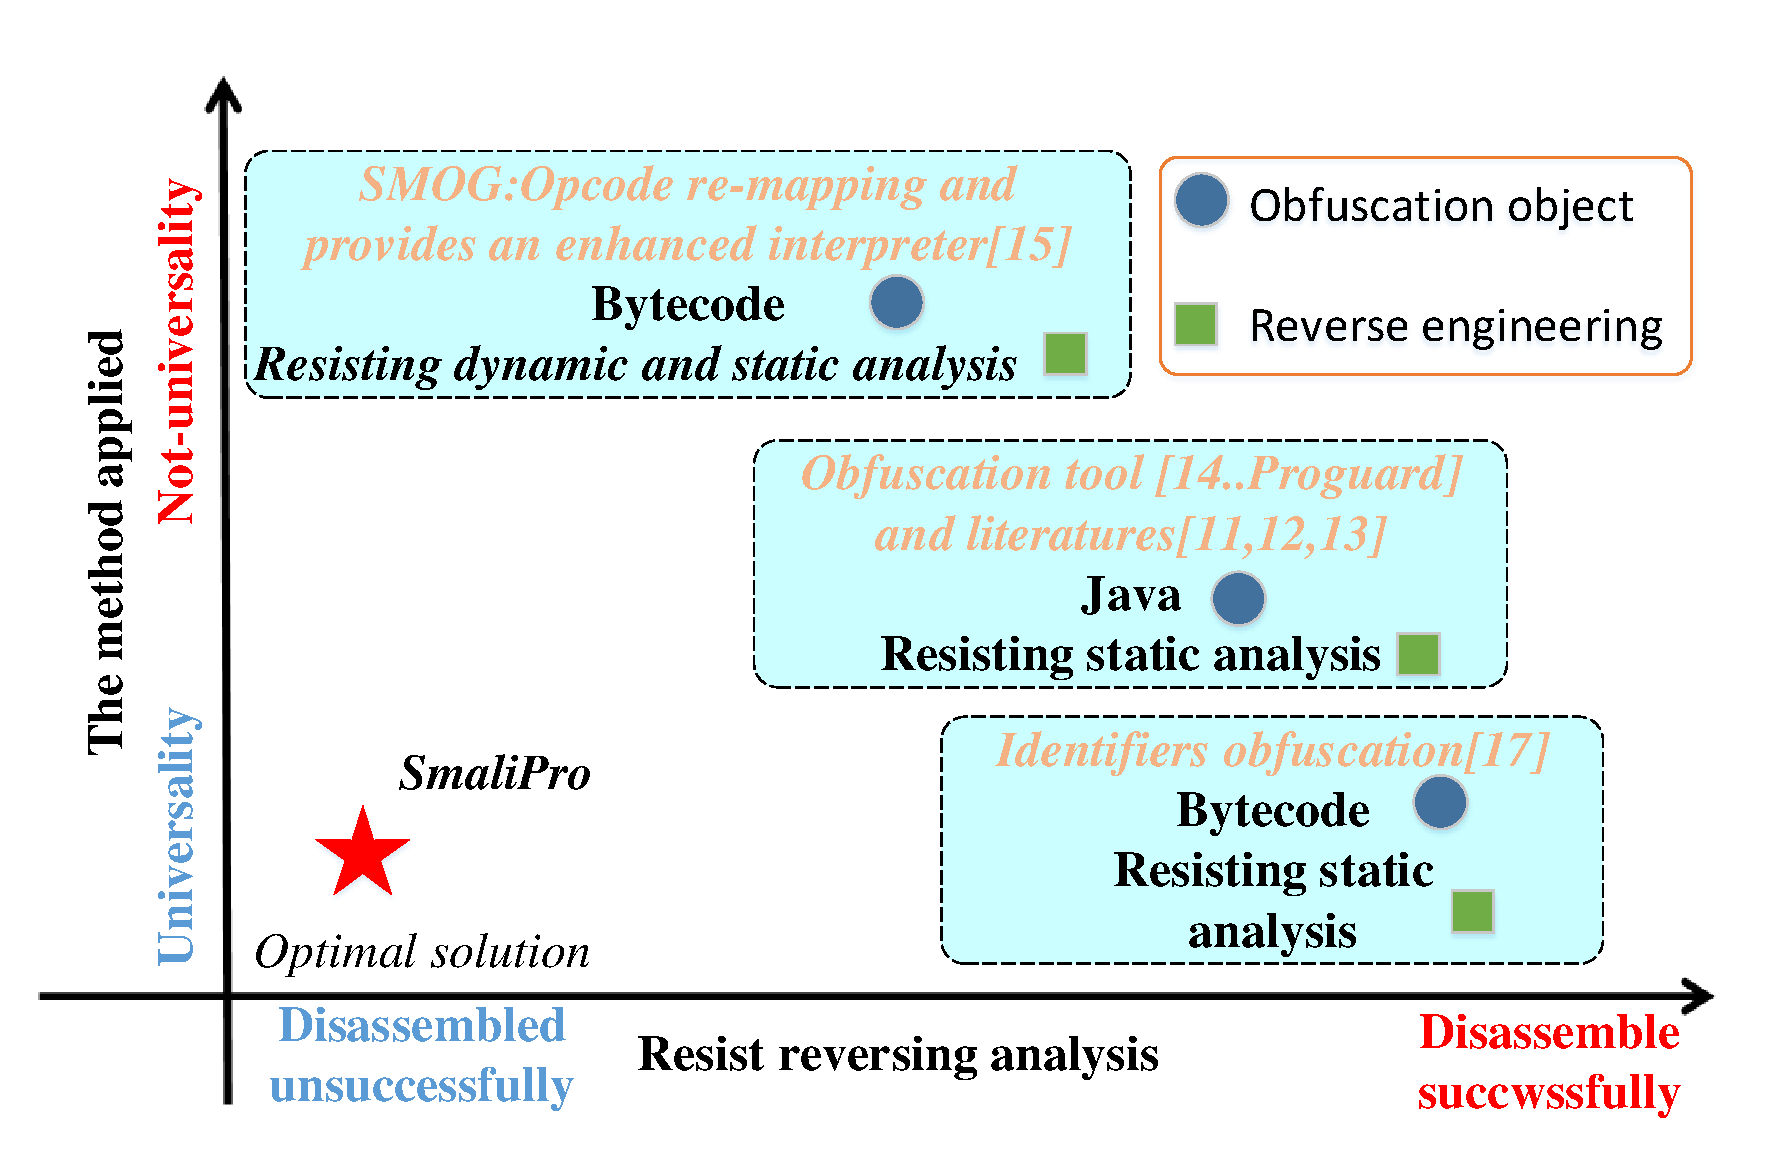
\includegraphics[width=0.8\columnwidth]{fig/fig1.pdf}\\
%  \caption{Design Space: comparing to related work.}\label{fig:Figure 1}
%  \FIXME{Change this into a table.}
%\end{figure}

%In this paper we propose SmaliPro, a comprehensive protection system based on obfuscated smali, an intuitive assembly language for Dalvik bytecode. Dalvik VM is one of the core part of the android mobile device platform and can support the form of .dex bytecode from Java source code. Its instructions are based on the architecture of register, so the constant pool was modified to use the index of 32 bits, which can simplify the interpreter. Therefore the constants and the return values of the function within smali code are stored in the 32-bit registers. When Dalvik VM performs the bytecode flow, it gets out the operand from the corresponding register in terms of the opcode, regardless of what the type of register is. According to this characteristic, we can confuse the data flow for the access procedure of register data, and combine opaque predicates\cite{13,17,18} technology to confuse the control flow. This method can resist decompiling and do not need the developer to provide the Java source code. The advantage of Our work is showing Figure\ref{fig:Figure 1}. We can see that the protection method will not only resist disassembled, but have universality.
%
%The core concept of SmaliPro is obfuscating the access procedure of constants in the registers. But the verifier component of Android runtime system(\emph{CodeVerify.app; DexVerify.cpp}) is referred to as VFY by Dalvik VM, which verifies the type of registers when loading the class. So our obfuscated application is not normally running. It is the challenge in this paper. In order to solve the problem, we use the dex dynamic loading technology and Dalvik runtime tampering technology, which is explained in Section 4.3.

In this paper, we present \ToolName, a novel bytecode level code obfuscation system for Android applications. \ToolName advances prior work in the following ways. Firstly, \ToolName performs code obfuscation on the bytecode level, so it does not require accessing to the source code and as a result the obfuscated code will not be optimized out by the compiler. Secondly, 
it requires no modification to the compiler and runtime environment. Hence the obfuscated code can run on any environment that supports the standard Android bytecode format. 
\ToolName exploit two key structures of the Android Dex bytecode definition to protect the program against dynamic code analysis: (1) all except for floating operands are based on a 32-bit register and (2) the instruction follows a function call is always used to retrieve the return value of the function. Our approach utilizes the register structure of Dex to pack two 32-bit operands into a single 64-bit data item, so that any attempt in decoding the protected operands will receive incorrect information. We leverage the calling conversion of Dex, to insert opaque predicates (i.e. code with complex logic but does not get executed) between instructions of the function call and return value retrieval. Doing so not only makes it harder for the attacker to obtain the return value, but also obfuscates the dynamic program behavior. By combining these two techniques, \ToolName provides stronger protection when compared to existing code obfuscation techniques that target at the source code or bytecode level, with little extra overhead.

We have evaluated our approach by using \ToolName to protect a number of
representative Android application operations. Experimental results show that
our approach can protect software against sophisticated reverse engineering
tools, including Jeb, Dex2Jar, dexdump and IDA pro, with less than
\FIXME{xx}\% increment in code size and runtime overhead.
This paper makes two specific contributions:
\begin{itemize}
\item It is the first work to exploit the register structure and calling convention of Android Dex for code protection;
\item It is the first byte-code level code obfuscation scheme that protects software against static and dynamic code analysis.

%\item This paper designs and implements a system SmaliPro based on smali code confusion, it does not need the developer to provide the Java source code and protects their intellectual property rights.
%\item SmaliPro aims at comprehensive protection of Android apps. It could resist not only static analysis but also dynamic analysis because the obfuscated bytecode cannot be correctly decompiled by the attacker.
%\item The performance overhead of obfuscated app is compared with the unprotected app, and the obfuscation method is evaluated by potency, resilience, availability and cost.
\end{itemize}

%\textbf{Structure of the paper:} We provide background and describe motivation in Section 2. Section 3 presents the overview of our system and Section 4 introduce the process of system implementation in detail. In Section 5, we discuss the potency, resilience and cost of the obfuscation method, and in Section 6 we deliberate evaluation of code obfuscation against current popular reverse tools and the overhead. Most relevant work in Android code obfuscation is discussed in Section7. Finally, the concluding remarks are given in Section 8. 
\section{Background}
%Next we give an overview on background information and the attacking scenario essential for understanding the key principles that underlie our proposed protection methods.

\subsection{Android Dex Bytecode}
Typically, Android applications are programmed using Java. The application source code is compiled to the Dex bytecode format which is then packed into a Android application package (APK) together with application resources (such as images and configuration files). 
The Dex bytecodes can be either dynamically interpreted (using the Dalvik VM before Android 5.0) or compiled into native machine code during installation by the Android Runtime since Android 5.0. Our approach only applies to the Dex bytecode without changing the Android VM or compilation process. Hence, our approach is portable across different Android versions. 





%and deployed as files with an ".apk" suffix, later called APK. It is basically a ZIP-compressed file and contains resources of the application like pictures and layouts as well as a dex file. This dex file, saved as "classes.dex", contains the program code in form of Dalvik bytecode. The content of the APK is also cryptographically signed, which yields no security improvement but helps to distinguish and confirm authenticity of different developers of Android applications. There are two Android virtual machine and the Dalvik VM was replaced by the Android runtime(ART). The difference between them is that ART virtual machine will translate the dex bytecode into native machine code when installing the application, so both virtual machines execute the same unmodified Dalvik bytecode file structure, instruction formats(smali), and constrains. Hence, our proposed obfuscation applies to apps run by both DVM and ART.
%Within the installation process, every installed application gets its own unique user ID by default. This means that every application will be executed as a separate system user. The execution process\cite{08} of an Android application is shown in Figure ~\ref{fig:Figure 3}.

\begin{figure}[!tbp]
  \centering
  % Requires \usepackage{graphicx}
  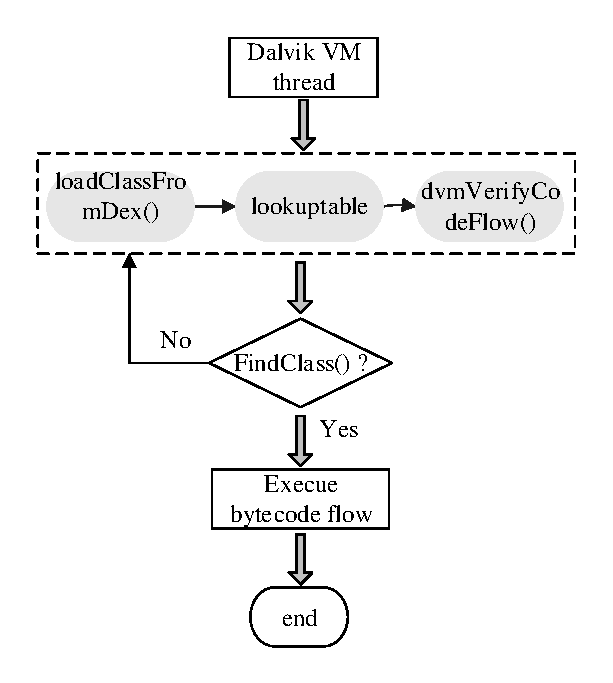
\includegraphics[width=0.8\columnwidth]{fig/fig3.pdf}
  \caption{The process of Dalvik VM execution. this figure presents the Dalvik VM how to execute an Android app\emph{(load, link, verify,run)}.}
  \FIXME{This diagram should go. Dalvik is dead. }
  \label{fig:Figure 3}
\end{figure}


\FIXME{We shouldn't talk of dynamic execution of Dex bytecodes. Again, this is because Dalvik is already dead!}

%In detail, the specific process is as follows:
%\begin{itemize}
%  \item \textbf{Load the Classes.} Firstly, Dalvik VM loads the class by function loadClassFromDex(), and when the classes have been successfully resolved, each class will have a ClassObject type of data structure in the runtime environment. Dalvik VM stores and searches all loaded classes by using gDvm.loadedClassed global hash table;
%  \item \textbf{Verify Bytecode.} Bytecode verifier verifies the loaded class by using function dvmVerifyCodeFlow();
%  \item \textbf{Find the main class.} Dalvik VM searches and loads main method class in gDvm.loadedClassed global hash table by using function FindClass( ). If it can't find the needed class, it will go back to load the class;
%  \item \textbf{Execute bytecode flow.} Initialize the interpreter by invoking function dvmInterpret( ) and execute the bytecode flow.
%\end{itemize}

 The Dex bytecode follows a stack machine where
operands of all operations are stored in a virtual 32-bit register. The only
exception is floating point operands which are always stored using a 64-bit
register. The other key structure of Dex is that function calls always follow by
an instruction to retrieve the return value
of the function. This is a key point where an attacker will focus on when attempting to trace the program control flow using dynamic code analysis.
The binary form Dex bytecode can be dissembled into Smali, a
human readable format of Dex.
To perform code protection, our approach first dissembles the Dex bytecode into Smali;
it then applies code obfuscation on Smali and assemble the obfuscated Smali code back into Dex bytecodes. 

Figure~\ref{} gives an example of the generated Smali code of a simple java
function. \FIXME{Here gives an example of how a Java function is compiled
into Smali. The example should show that the operands are stored in a 32-bit
register and the function call is always follows by an instruction to
retrieve the return value}.



%
%\textbf{smali code.} We can disassemble the contents of the app and generate folder in disassembling project directory, using the android-apktool, which contain all the disassembled smali\cite{03} files. These files will be generated according to the package hierarchy corresponding directory and all classes generate independent smali files in the corresponding directory of the program\cite{20}.
%
%The smali code is a instruction language of Dalvik VM, which is register-based, and frames are fixed in size upon creation. Each frame consists of a particular number of registers(specified by the method)as well as some adjunct data needed to execute the method. When used for bit values(such as integers and floating point numbers), registers are considered 32 bits wide. Adjacent register pairs are used for 64-bit values, such as double and long numbers. All variables of smali code are stored in registers. For example, in the instruction "const-wide v0, 0x0000000400000003 ", it is a definition of the long number, indicating that it operates on wide(64 bit) data, and "v0,v1" is the destination register.


\subsection{The Attacking Model}
%Reverse engineering is the necessary condition that Android applications are repackaged or tampered by attackers. This process aims at enabling an analyst to understand the concrete relation between implementation and functionlity of the program. In this paper we focus on resisting the decompiling process because this is the fundamental step in reverse engineering due to the fact that most of the other processes are based on the decompiling process.

Figure~\ref {fig:Figure 2} illustrates a representative attacking scenario for Android applications. We use this attacking model to evaluate our approach in this paper. To perform the attack, an adversary first extract the Dex file from application APK. The attacker will then xxx.
\FIXME{I have no idea why the attacker will translate dex bytecode into Java code?}
%In recent years, the attackers usually achieve their malicious behaviors. Firstly, they can successfully decompile .dex into .java, which is java source code.But they will not analyze smali code that is after disassembling, because of enormous and complex grammar than Java source code. Therefore, an attacker locate the critical sections from all over the java source codes quickly, then analyze the main function within the smali file\cite{04} or .so native library based on the previous position.The process is as shown in Figure~\ref{fig:Figure 2}.


\begin{figure}[!tbp]
  \centering
  % Requires \usepackage{graphicx}
  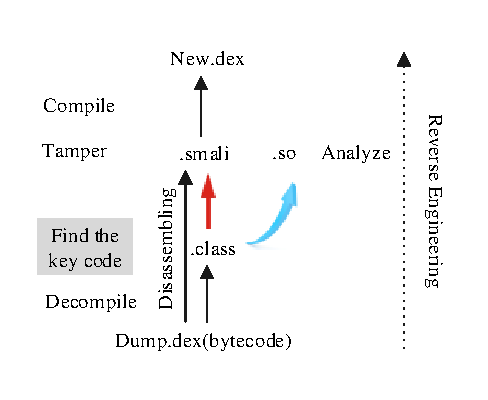
\includegraphics[width=0.8\columnwidth]{fig/fig2.pdf}
  \caption{Reverse engineering. The process that attacker was cracked a app is shown in the figure. }\label{fig:Figure 2}
\end{figure}

We can analyze a instance about online ordering app from Android Open Source Software Community. Firstly, we can see that two variables within java source code is defined in the code of ordering. It is the int-type of the number of clicks and purchase quantity and shown in the following:


\begin{lstlisting}[language={[ANSI]C}, backgroundcolor=\color{backcolour},
numbers=left,numberstyle=\tiny,keywordstyle=\color{blue},commentstyle=\color{red!50!green!50!blue!50}][6pt]
private int CLICK_NUM = 0;
private int buyNum = 0;
\end{lstlisting}

\noindent According to the location, we can quickly find it in the smali code. It is shown in following:

\begin{lstlisting}[language={[ANSI]C}, backgroundcolor=\color{backcolour},
numbers=left,numberstyle=\tiny,keywordstyle=\color{blue},commentstyle=\color{red!50!green!50!blue!50}][6pt]
const/4 v7, 0x0
.local v7, CLICK_NUM:I
const/4 v8, 0x0
.local v8, buyNum:I
\end{lstlisting}

\noindent  If they didn't be protected, the attackers can find their location and then modify their initial value to steal the user's money. In order to resist this kind of attack, we processed a method through obfuscating variables of being stored in registers.


\section{Overview of Our Approach}
As depicted in Figure~\ref{fig:Figure 4}, the system is proposed as a software protection system within which an obfuscation engine and solving the conflict problem. It mainly obtain three part.

At the first part, we are mainly introduce to how to obfuscate the smali code. The basic idea is confusing the data-flow for the access procedure of register data, and combining opaque predicates technology to confuse the control-flow.

The next step, because our obfuscation method would cause problems of the register-type conflict, we should make the executable .dex file normally execute by the Dalvik VM. So we need to modify the .dex file ,which is  explained in Section 4.3.

Lastly, we will utilize the dex dynamic loading technology to load the above .dex file, but some bytecode is nop after the class being loaded, so Dalvik runtime tampering technology is used to solve the problem. Meanwhile, To illustrate this, we firstly analyzed the exact nature of the problem, and then describe the details process that is to implement normal running.


\begin{figure}[!tbp]
  \centering
  % Requires \usepackage{graphicx}
  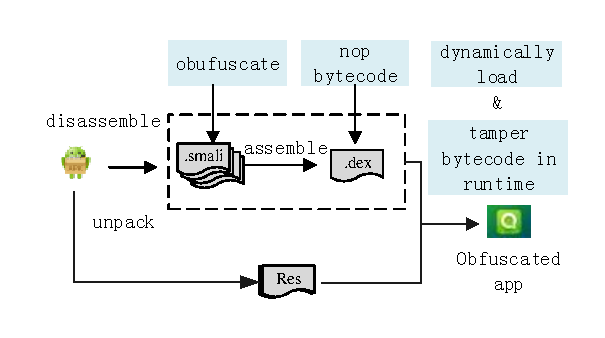
\includegraphics[width=1\columnwidth]{fig/fig4.pdf}
  \caption{Workflow of the SmaliPro system. we can see three part, obfuscate the smali code ,nop bytecode within the .dex file, and dynamic load and runtime tamper, which is the background of the light-green.}\label{fig:Figure 4}
\end{figure}


\section{Implementation details}
In this section, we describe some implementation details for the obfuscation techniques, starting with obfuscating engineering of our approach.
\subsection{Obfuscate the value of register}
Dalvik VM's instructions based on the architecture of register and the constant pool is modified to use the index of 32 bits, which can simplify the interpreter. Therefore the constants within smali code  are stored in the 32-bit registers. According to this characteristic we can confuse the access procedure of constants and control flow, that is data flow obfuscation and control flow obfuscation.

Dalvik VM get the operand from the corresponding register directly based on the type of operation code when perform bytecode flow, regardless of what the type of register is, so we can obfuscate from two aspects. On the one hand, because the constants of the long  and double in smali code are 64-bit, they are stored in the two adjacent 32-bit registers, so we can use a long constant instead of the two constants respectively stored in two 32-bit registers . On the other hand, we will confuse a instruction of capturing the return value of an object reference for a instruction of capturing the return value. The two methods on the above is to confuse on the data access, so that it can make the compiler tools puzzled.

Confusing the control flow is an effective way. its principle is to hide or modify the real control process that adopt various technical, which is to adjust the program structure and the execution path, or to add the opaque predicates and so on to increase the difficulty of the compiler, so that it can prevent the attacker to analysis the control flow of the program\cite{12}.

In this paper, we propose a obfuscation method by inserting reinforced opaque predicates\cite{07}. The first step is to judge the position where to insert, which was conducted on the basis of process analysis. Invoking the key function(\emph{self-define}) is very important modules of program, so we can insert the location of reinforced opaque predicates where is between the instruction of invoking the key function and  the accessing returned value, and the process is shown in Figure~\ref{fig:Figure 5}. For example, the function of purchasing equipment function is very critical in the game and its returned value is usually analyzed by the attacker. If the developer take such protection method, the attackers can't get the return value. This way not only increase the complexity of control flow, but data flow.

\begin{figure}[!tbp]
  \centering
  % Requires \usepackage{graphicx}
  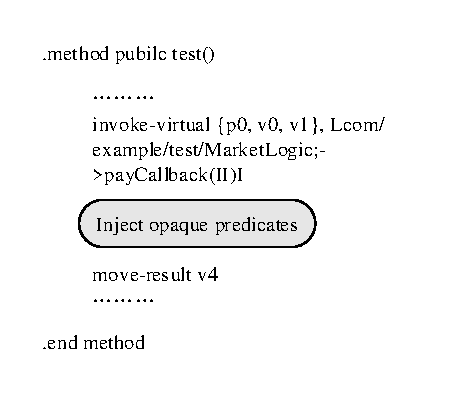
\includegraphics[width=0.8\columnwidth]{fig/fig5.pdf}
  \caption{Control obfuscation. In order to obfuscate the control-flow, we will inject the opaque predicates between two instructions that are invoking and capturing the return value.}\label{fig:Figure 5}
\end{figure}
\subsection{Register type-conflict problem}
Let us consider a small Obfuscated smali method, which is the method of adding two numbers.

\begin{lstlisting}[language={[ANSI]C}, backgroundcolor=\color{backcolour},keywordstyle=\color{blue},commentstyle=\color{red!50!green!50!blue!50}]
.method public static add()I
    const-wide v0, 0x0000000300000002
    add-int v2 , v0,v1
    return v2
.end method

\end{lstlisting}

\noindent The long variable is stored in v0 and v1. When they are to be added, the Dalvik VM will terminate the app and output the following type-conflict error messages to logcat:
\begin{lstlisting}[language={[ANSI]C}, backgroundcolor=\color{backcolour},keywordstyle=\color{blue}]
VEY: register1 v0 type 19, wanted 17
VEY: register1 v1 type 20, wanted 17
VEY: rejecting opcode 0x90 at 0x0008
VEY: rejected Lcom/example/****/****;
.add()I
Verifier rejected class Lcom/example/
****/****;
Class init failed in newInstance

\end{lstlisting}

We can see this register-type conflict problem from the static program analysis'viewpoint follows. The verifier module\cite{35,36} to perform a register type analysis each method within a class prior to running it, and ensure that there is no type conflict. Should it the register with two diffirent types at the same method when loading the class, it will then report the register-type conflict problem as shown above.

Given this issue, we thus need to find a solution that will bypass the verifier of the evaluated Android runtime systems from deducing any false type conflict in otherwise correctly obfuscated apps.




\subsection{App execution}
As shown in Figure~\ref{fig:Figure 3}, Dalvik VM verifies the validity of instructions when loading the class, for example, verifying the type of the registers. so executing an obfuscated app must bypass the process of the verifier.To address the problem, we can do the following three things.

\begin{enumerate}[leftmargin=*]
\item[(i)] First of all, we will recompile the obfuscated smali into a .dex file . Then the bytecode of each obfuscated method which is in the .dex file can be stored in the ObjMethod structure of showing in Figure~\ref{fig:Figure 6}. At last, we will fill the zero bytecode in the obfuscated method and get a new.dex file. This way resist static analysis successfully.

\item[(ii)] In order to load the executable file new.dex utilizing the technology of loading dex dynamically, we develop our own customized Classloader to load all the classes in this dex file, before which the default Classloader in the API layer should be replaced to ensure the normal execution of the real dex file.

    There exists a system component called Application[14] in Android frame. it will initialize several global variables when establishing Application(i.e. before launching app ),  and all the Activity within the same app can access the value of these variables. Usually, system will develop an Application automatically and we don't need to develop it specifically, so through designing customized class ProxyApplication that extends  Application, the default Classloader in the system will be replaced by the customized MyDexclassloder when initiating ProxyApplication. Moreover, we should configure ProxyApplication in the ApplicationManifest.xml file as folllows:
    \begin{lstlisting}[language={[ANSI]C}, backgroundcolor=\color{backcolour},keywordstyle=\color{blue!70},commentstyle=\color{red!50!green!50!blue!50}]
    <application
      Android:name="ProxyApplication"
    </application
    \end{lstlisting}


\item[(iii)] In order to bypass verification of Dalvik VM for instructions(i.e. register types), we utilize  the technology of dynamically loading. As bytecode in the obfuscated  methods  in new.dex is a zero sequence after loading new.dex, we need to fill the obfuscated bytecode in the corresponding location in the memory before execution.

    \par When running an Android appication, it will load dex file and parse the dalvik bytecode that is executed by Dalvik VM. We reads or writs the byte flow when running the app with the aid of the JNI component\cite{15}, as there isn't a direct method to achieve this compared to X86 and ARM frame due to limited instruction sets of DVM. Native library and Dalvik VM owe the same priority as they are in the same process, so we can utilize JNI to call methods in native library to achieve the modification for Dalvik bytecode.

    The address of dex in the memory after loading can be acquired through DexFile class in Android system. According to the address, we can acquire the memory address of the obfuscated methods via parsing the dex structure, then fill in the corresponding memory address with the corresponding  bytecode stored in the ObjMethod structure to ensure correct system execution.
\end{enumerate}

\begin{figure}[!tbp]
  \centering
  % Requires \usepackage{graphicx}
  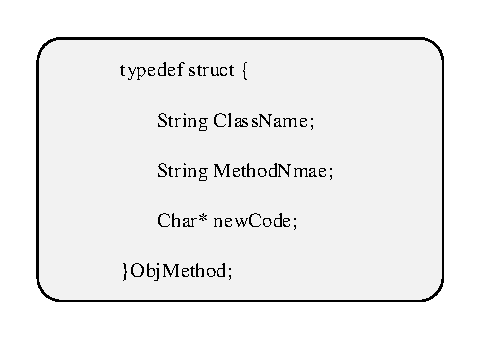
\includegraphics[width=0.8\columnwidth]{fig/fig6.pdf}
  \caption{The structure of ObjMethod. It is used to store the bytecode of the obfuscated method within the .dex file. The bytecode backfill the memory after the class loaded}\label{fig:Figure 6}
\end{figure}
\section{Obfuscation evaluations}
\subsection{Evaluations criteria}
Collberg\cite{16} gives an accurate definition on code obfuscation: The i is one of all possible inputting set \emph{I} which is in the program \emph{P}. If and only if it is $\forall$ \emph{i:T(P)(i)=P(i)}, we can just think that the transition of the confusion was correct. The obfuscation method is evaluated from potency, resilience and cost by Collberg at al.

Let \emph{T} be a behavior-conserving transformation, such that \emph{P $\underrightarrow{T}$ P'} transforms a source program \emph{P} into a target program \emph{P'}.

\emph{T$_{pot}$(P)}, the potency of \emph{T} with respect to a program \emph{P}, is a measure of the extent to which \emph{T} changes the complexity of \emph{P}. Let \emph{E(P)} be the complexity of \emph{P}.  It is defined as

 \begin{equation}\emph{T$_{pot}$(P)=E(P')/E(P)-1}\end{equation}

 \noindent T is a potent obfuscating transformation if \emph{T$_{pot}$(P)>0}.

\emph{T$_{res}$(P)} is the resilience of \emph{T} with respect to a program \emph{P}. \emph{T$_{res}$(P)=one-way} if information is removed from \emph{P} such that \emph{P} cannot be reconstructed from \emph{P'}. Otherwise,

 \begin{equation}\emph{T$_{res}$(P)$\triangleq$ Resilience(T$_{Deobfuscaor effort}$,T$_{Programmer effort}$)}\end{equation}

\emph{T$_{cost}$(P)} is the extra execution time/space of \emph{P'} compared to \emph{P}. that is to say

\begin{equation}\emph{T$_{cost}$(P)=Cost(C$_{time}$ , C$_{size}$)}\end{equation}

\subsection{Evaluations based on smali code obfuscation}
Potency. The proposed code confusion method includes both control obfuscation and data obfuscation. In data obfuscation, we can obfuscate the instructions of accessing the values from the registers and calling method that its returned value is object type. In control obfuscation, in order to resist attacker to accessing the returned values which is after calling the key function, we will insert the opaque predicate between two instructions that are calling and accessing returned value. The above two kinds of method can both resist the attacker to acquire correct program code and increase the complexity of the control flow. Thus, the method of proposed has good strength.

Resilience. The obfuscated program has been analyzed from the point of reverse analysis. For example, the attacker can't accessing correct instructions and analyzing logical construction of program. As shown in Figure~\ref{fig:Figure 7}, decompilation process is failure and control flow becomes very complicated. so the method of proposed has strong slastic.

Cost. The function's time complexity is O(1) after being obfuscated. Firstly, inserting opaque predicate and modifying the instruction format is not to change polynomial of the complexity. Secondly, dex dynamic loading and backfilling the bytecode both increasing little time, but as shown in Figure \ref{fig:Figure 8}, only the first launching time increases more. In space consumed, we will only insert opaque predicate into invoking the key function and obfuscated instructions is short. Thus this method has little effect on the time and space consumed.


\begin{figure}[!tbp]
  \centering
  % Requires \usepackage{graphicx}
  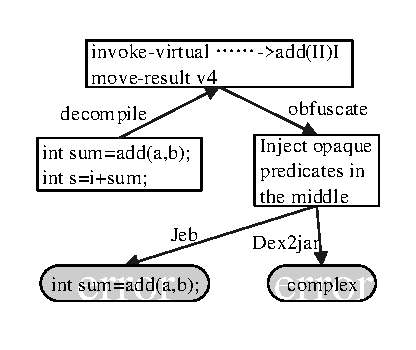
\includegraphics[width=0.8\columnwidth]{fig/fig7.pdf}
  \caption{The case of reversing engineering. When we inject the opaque predicates after invoking the \emph{add()} method, the attacker can't capture the return-value \emph{sum.}}\label{fig:Figure 7}
\end{figure}
\section{Experiment results}
Based on the deep research in SmaliPro, as shown in Fig.2, this paper designed and implemented a prototype system. It can resist the static analysis and dynamic analysis of the process of the reverse engineering. All experiment are conducted on the Android virtual decice of Android Version 4.2, which has 512M RAM, and 256M internal storage.

To measure the performance overhead and effectiveness of SmaliPro, we first selected four typical applications which have different instructions as test case. These four apps are listed in Table~\ref{tab:Table 1}.

\begin{table}[htbp]
  \centering
  \rowcolors{2}{gray!25}{white}
  \begin{tabular}{c c}
  \toprule
  Test case & The characteristics of the instruction\\
  \hline
  \hline
  Long.apk & Define 32-bits constant\\


  Re\_objapk & Returned value of the reference type\\


  Key\_fuc.apk & key function(self-defined)\\


  Compre.apk & All the above\\
  \bottomrule
  \end{tabular}
  \caption{A list of apps we selected to test. Column 2 represent the type of instructions of four typical Android apps. }\label{tab:Table 1}
\end{table}

\subsection{Effectiveness}
The main purpose of this paper is to protect the executable code of the application, and make it not be easy analyzed by attacker. The below from two aspects of resisting static and dynamic  analysis analyze the effectiveness of the protection method based on confusion of smali code.

The some bytecode within executable file is a zero sequence before executed bytecode flow by DVM. So when attackers want to statically analyze the logical structure of the program, they can't acquire correct bytecode. Before the app running the attackers dump the bytecode through dynamically analyzing, this way is the same with resisting static analysis. If running, they will dump the obfuscated bytecode, which isn't correctly decompiled, as shown in Figure~\ref{fig:Figure 5}.

In order to the effectiveness of the obfuscated method, we will also utilize reversing tools to reverse executable code of the application. The experiment results is shown in Table~\ref{tab:Table 2}.

\begin{table}[htbp]
  \centering
  \rowcolors{2}{gray!25}{white}
  \begin{tabular}{c c c c c}
  \toprule
  Test case & Jeb & Dex2Jar & dexdump & IDA pro\\
  \hline
  \hline

  Long.apk  & $\times$ & $\times$ & $\ast$ & $\ast$\\


  Re\_objapk & $\times$ & $\times$ & $\ast$ & $\ast$\\


  Key\_fuc.apk & $\times$ & $\ast$ & $\times$ & $\ast$\\


  Compre.apk & $\times$ & $\times$ & $\times$ & $\ast$\\
  \bottomrule
  \end{tabular}
   \caption{The results of analysis by reversing tools. $\times$ represent that the code after reversing is wrong. $\ast$ represent that it becomes very complicated}\label{tab:Table 2}
\end{table}

\subsection{Performance overhead}
We measured the performance overhead of SmaliPro by comparing the executable file size, memory use and launch time of applications before and after obfuscated by SmaliPro.

Table~\ref{tab:Table 3} illustrates the file size and memory use changes of applications before and after obfuscated. we can see that the dex file size increases more than 300 bytes. This increase in file size is mainly due to the packer dex file that is used to load really dex file and inserting the instructions. The results are not obvious because the application size we selected is relatively small and little difference.

We will describe that memory costs are mainly caused by the paker dex file and native library. But current mobile devices tend to provide more RAM, you can ignore the costs.

To measure the app response delay after being protected by SmaliPro, we compared the app launch time for the first, second, third, and fourth run before and after obfuscated. To make it more precisely, we did each experiment 20 times and used the average value as a final reference. The launch time of four test case is listed in Table~\ref{tab:Table 4}.

Figure~\ref{fig:Figure 8} shows the app launch time changers at each time. We can see that the time increase at the first launch, which is mainly caused by: 1) running the obfuscated application needs to replace Classloader; 2) Before running we must find the obfuscated method in the corresponding memory address through parsing the structure of the dex file and then fill the bytecode that is stored in ObjMethod in the address. These classes and libraries will be loaded at the application's first execution and will be kept in the memory so long as the system resources are sufficient. Thus, they do not need to be loaded again in the app's latter launch, which is the reason why they all show a similar launch time as the unprotected apps at the latter launch.

\begin{figure}
  \centering
  % Requires \usepackage{graphicx}
  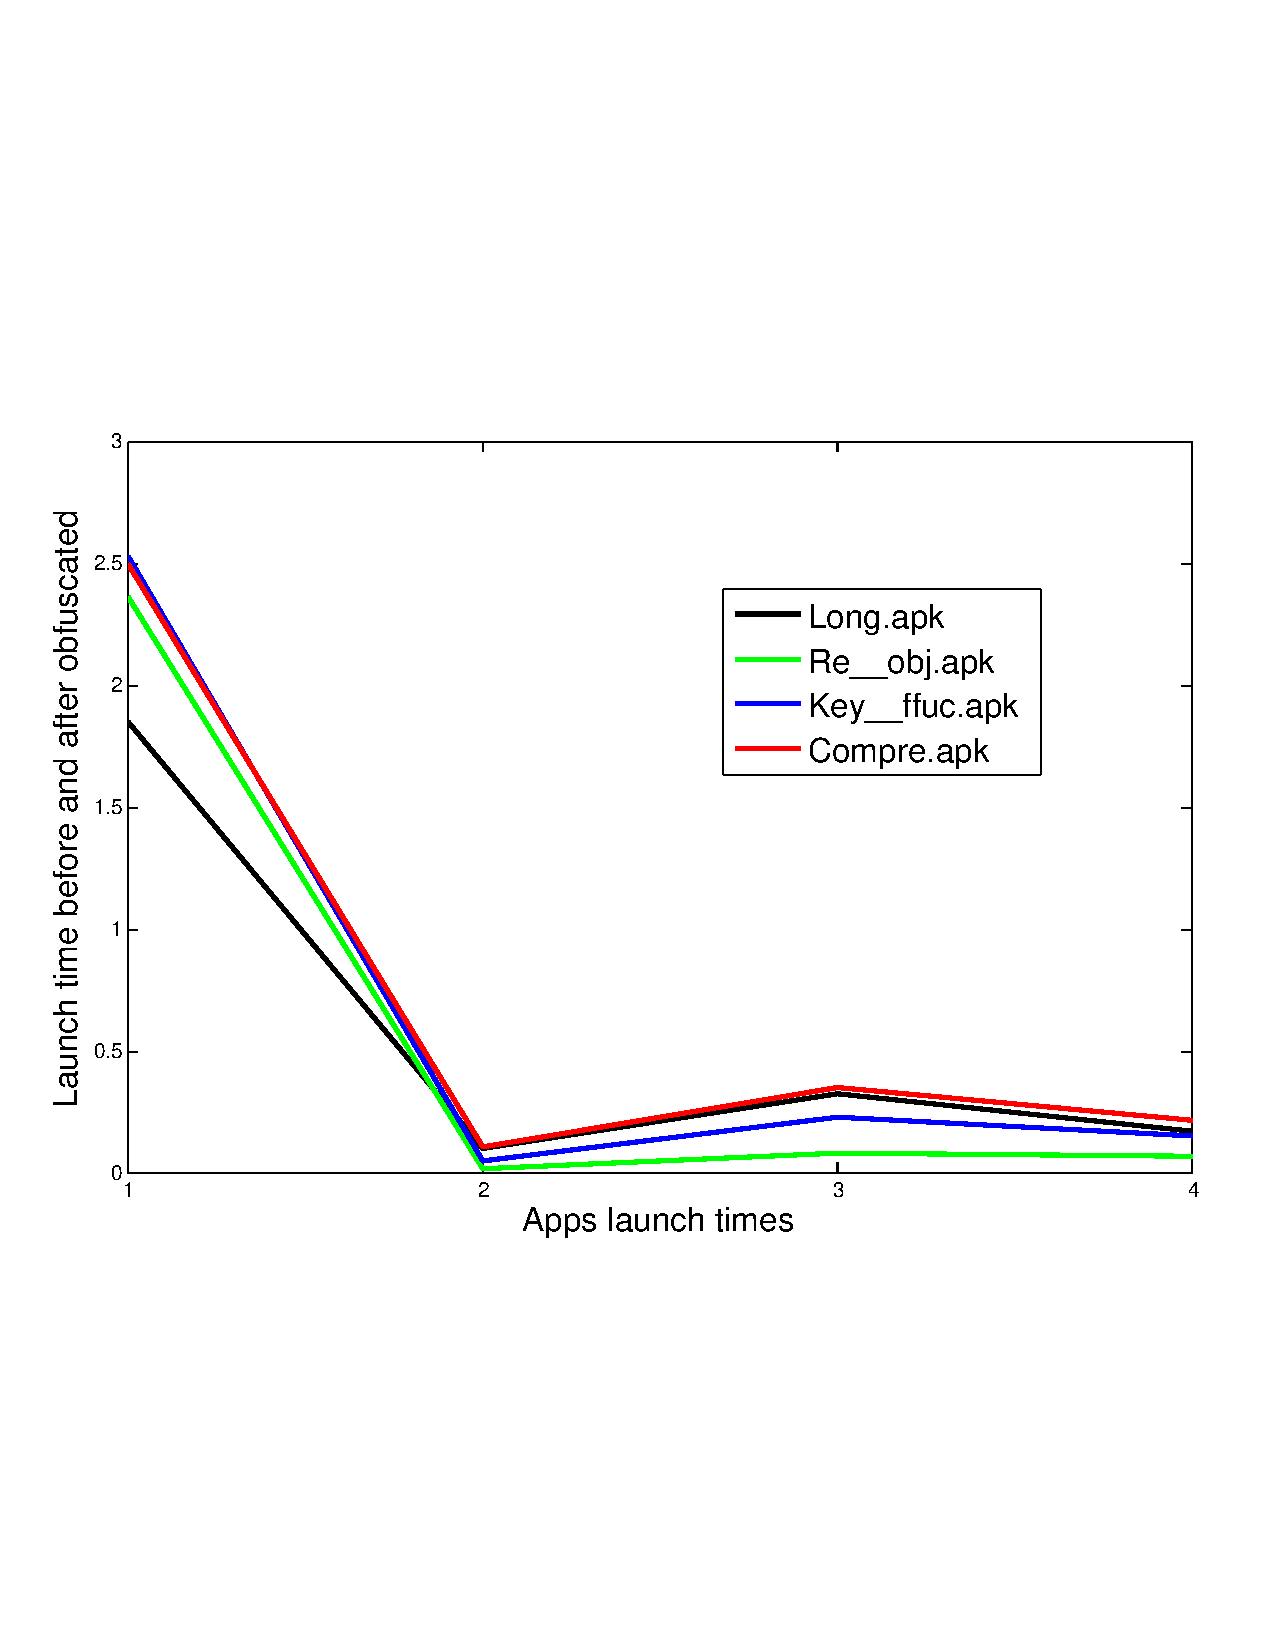
\includegraphics[width=0.8\columnwidth]{fig/fig8.pdf}\\
  \caption{Describe the changes of launch time D-value. Compare to the first ,second, third ,and fourth launch time D-value before and after obfuscated. we can see only that the time significantly increase at the first launch  }\label{fig:Figure 8}
\end{figure}


\begin{table}[htbp]
  \centering
  \begin{tabular}{c c c c c}
  \toprule
  \multirow{2}{*}{Test case} & \multicolumn{2}{c}{Dex file size (bytes)} & \multicolumn{2}{c}{Memory use(KB)}\\
  \cline{2-5}
  \cmidrule{2-5}

  & Before & After &  Before & After\\
  \hline

  Long.apk & 449040 & 462328 & 4320 & 5858\\
   \rowcolor{mygray}


  Re\_obj.apk & 449080 & 462392 & 4072 & 7082\\


  Key\_fuc.apk & 449176 & 462483 & 4349 & 6248\\

\rowcolor{mygray}
  Compre.apk & 449232 & 462556 & 4866 & 6406\\
  \bottomrule
  \end{tabular}
  \caption{Comparison of file size and memory use before and after obfuscated. Column 2 and Column 3 represent the size changes of dex file before and after obfuscated. Column 4 and Column 5 shows the size changes of memory use.}\label{tab:Table 3}
\end{table}

\begin{table*}[htbp]
  \centering
  \begin{tabular}{c c c c c c}
  \toprule

  \multicolumn{2}{c}{Test case} & Long.apk & Re\_obj.apk & Key\_fuc.apk & Compre.apk\\
  \hline
   \hline
  \multirow{2}{*}{First(s)} & Before & 2.175 & 2.249 & 2.124 & 2.912\\
  & After & 4.027 & 4.612 & 4.677 & 5.412\\
  \hline


  \multirow{2}{*}{Second(s)} & Before & 0.939 & 0.923 & 0.844 & 0.911\\
  & After & 1.027 & 0.942 & 0.892 & 1.017\\
  \hline

  \multirow{2}{*}{Third(s)} & Before & 0.845 & 0.882 & 0.797 & 0.891\\
  & After & 1.171 & 0.959 & 1.024 & 1.238\\
  \hline

  \multirow{2}{*}{Fourth(s)} & Before & 0.823 & 0.862 & 0.781 & 0.887\\
  & After & 0.994 & 0.928 & 0.934 & 1.099\\

  \bottomrule
  \end{tabular}
   \caption{Launch time(in seconds) of four apps for the four times launch before and after obfuscated.}\label{tab:Table 4}
\end{table*}
\section{Related work}
Obfuscation is a useful and cost effective technique and it doesn’t require any special execution environment. Moreover it is believed to be more effective on Android system\cite{21,22}. Patrick Schulz in his work “Code Protection in Android”\cite{20} discusses some possible code obfuscation methods on the Android platform using identifier mangling, string obfuscation, dead code insertion, and self modifying code. Ghosh et al.\cite{23} have discussed a code obfuscation technique on the Android platform that aims at increasing the complexity of the control flow of the application so that it becomes tough for a reverse engineer to get the business logic performed by an Android application. Kundu has also worked on some obfuscation techniques like clone methods, reordering expressions and loops, changing the arrays and loop transformations\cite{24}.

There are various Android obfuscation tools available in the market, such as Proguad\cite{09}. But the current Android obfuscation tools seem to still lack the combination of complex control-flow and data-flow obfuscation techniques. In \cite{06,07,08} authors presents confusion scheme and algorithm of Android oriented software Java code, combined with the algorithm and improved insertion branch path and flattening the excess flow of control of these two kinds of control flow obfuscation method.

Junliang Shu et al. proposed SMOG\cite{10}, a comprehensive executable code obfuscation system to protect Android app. The obfuscation engine is at software vendor's side to conduct the obfuscation on the app's executable code, and then release the obfuscated app to the end-user along with an excution token. SMOG will also modify the code of DVM interpreter. Noor et al.\cite{26} present a protection scheme based on obfuscation, code modification and cryptographic protection that can effectively counter reverse engineering.

Vivek Bala et al.\cite{27} analyzed the need for potent control-flow based obfuscation so as to help protect Android apps. they also have described the design and implementation of three control-flow obfuscations for Android apps at the Dalvik bytecode level, which go beyond simp control-flow transformations used by exiting Android obfuscators. The register-type conflict problem raised by the Android runtime system has also been addressed by means of our type separation technique. 
\section{Conclusion and future work}
To deal with the problems that Android application is easily to be tempered and repacked, this paper proposes a protection method based on obfuscating smali code. We have analyzed the related work about protecting the code of Android apps in recent year. We also have described the design and implementation of confusing the data flow for the access procedure of register data, and combining opaque predicates technology to confuse the control flow. This method can resist decompiling. Meanwhile, we evaluate the potency, resilience and cost of the code obfuscation method. Experimental result demonstrates excellent performance of the effectiveness and low cost.

The protection method presented in this paper has some limitations as well. It can only be used some specific instructions formant and not be used at large scale. Our proposed method does not protect the resources and native library .so of an Android app and protects only the dex file.

In the future work, we will utilize the technology of control-flow platting to confuse the control-flow of an program and protect native library .so to strengthen the protection and increase difficulty in reverse engineering.
\section*{Acknowledgements}
This work was partial supported by projects of the National
Natural Science Foundation of China (No. 61373177, No.
61572402), the Key Project of Chinese Ministry of Education
(No. 211181), the International Cooperation Foundation of
Shaanxi Province, China (No. 2013KW01-02, No. 2015KW-
003, No. 2016KW-034), the China Postdoctoral Science Foundation (grant No. 2012M521797), the Research Project of
Shaanxi Province Department of Education (No. 15JK1734),
and the Research Project of NWU, China (No. 14NW28),

\bibliographystyle{abbrv}
\bibliography{reference}

\end{document}
